\documentclass{article}
\usepackage[utf8]{inputenc}
\usepackage[english,serbian]{babel}
\usepackage{indentfirst}
\usepackage{verbatim}

\usepackage{xcolor}
\usepackage{graphicx}
\renewcommand{\figurename}{Slika}
\graphicspath{ {./Slike/} }

\title{INFORMACIONI SISTEMI\\Online Novinarska Agencija}
\author{
David Nestorović 1083/22\\
Momčilo Knežević 1087/22
}

\date{Beograd, 2022.}

\begin{document}

\maketitle

\newpage

\tableofcontents

\newpage

\section{Uvod}
\indent Rad predstavlja projekat iz predmeta Informacioni sistemi na master studijama Matematičkog 
fakulteta. Rad opisuje informacioni sistem online novinarske agencije. \\
\indent Obzirom da živimo u vremenu gde su informacije ključne za svakodnevno funkcionisanje, ovakav sistem omogućuje da se informacije pravovremeno i efikasno šire tako da budu dostupne što većem broju ljudi.  Ideja je, da se u eri pametnih telefona, uspostavi direktna veza između novinarskih agencija i korisnika.

\section{Analiza sistema}
Informacioni sistem Online novinarske agencije omogućava pravovremeno širenje informacija iz raznih sfera interesovanja, putem interneta. Tok informacija kretao bi se od novinarskih agencija ka čitaocima. Pored toga, bitan aspekt sistema bilo bi i  procesuiranje dobijenih vesti od strane urednika agencije. Takođe bilo bi poželjno da sistem omogućava neki vid povratne informacije od korisnika ka samoj agenciji (komentari, ocene članaka...)  \\
\indent Činioci sistema u opštem slučaju su: \\
\indent \textbf{Novinar} - čija je uloga da prikuplja i šalje vesti, o nekom događaju, uredniku agencije u kojoj je zaposlen. Svaka vest, trebala bi da odgovori na šest novinarskih pitanja: Ko? Šta? Kada? Gde? Zašto? Kako? Pored toga, vest može sadržati i fotografiju i/ili video snimak koji bi dodatno privukli pažnju korisnika. \\
\indent \textbf{Administrator} - ima ulogu da održava bazu i rukovodi kreiranjem(odobrava) i brisanjem korisničkih naloga.
\\
\indent \textbf{Urednik} - čija je uloga da procesuira dobijene vesti, donese odluku koje od njih će bit objavljene, i vrši korekcije ukoliko je to potrebno. Pored toga, on može obavljati i funckiju novinara, odnosno može i sam pisati vesti. U pogledu interakcije sa čitaocima, uloga urednika je i da vrši recenziranje pristiglih komentara korisnika. \\
\indent \textbf{Čitalac} - koji koristi sistem za čitanje objavljenih vesti. Pored toga, registrovani čitaoci mogu postavljati komentare, davati ocene za objavljene vesti, i imati uvid u komentare drugih čitalaca. 
\\
\indent Na Slici 1 se nalazi dijagram koji prikazuje učesnike sistema i njihove akcije.

\newpage

\begin{figure}[htbp!]
\centering
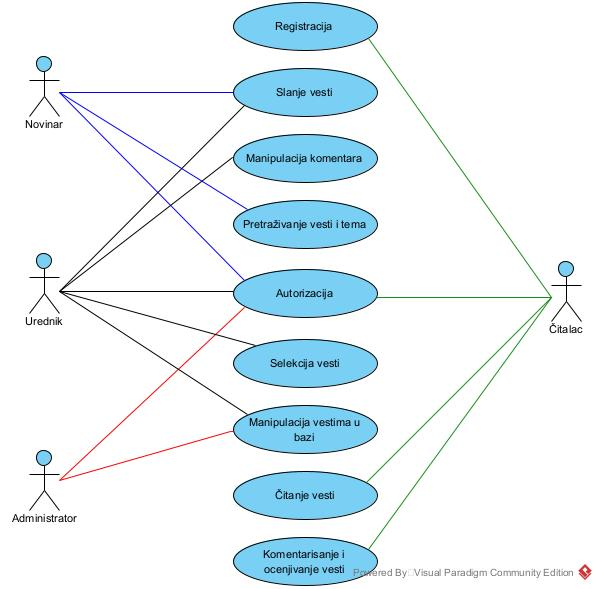
\includegraphics[scale=0.7]{Slucajevi_upotrebe.jpg}
\caption{Slučajevi upotrebe}
\label{slk:dtp}
\end{figure}

\newpage

\begin{figure}[htbp!]
\centering
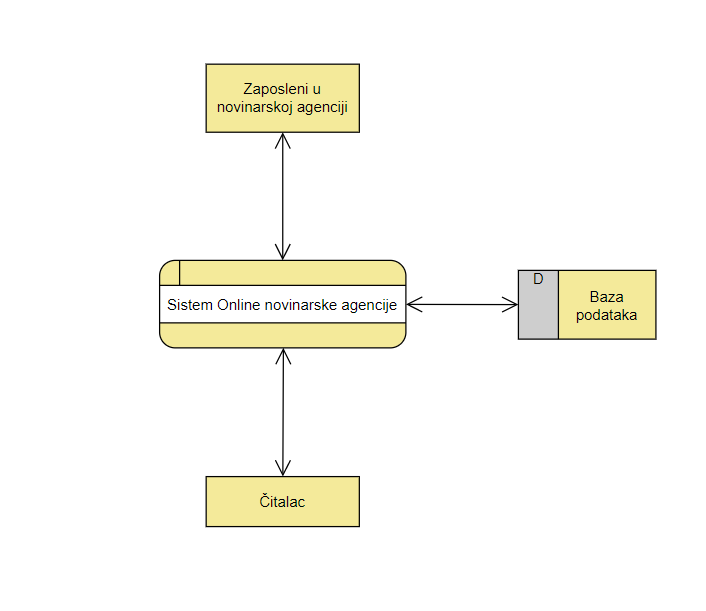
\includegraphics[scale=0.7]{Dijagram_konteksta.png}
\caption{Dijagram konteksta}
\label{slk:dtp}
\end{figure}

\newpage

\section{Slučajevi upotrebe}
\indent Posmatrani sistem identifikuje sledeće slučajeve upotrebe:
\begin{itemize} 
\item Registracija
\item Autorizacija 
\item Slanje vesti
\item Pretraživanje vesti i tema
\item Manipulacija vestima u bazi
\item Selekcija vesti 
\item Manipulacija komentara
\item Čitanje vesti
\item Komentarisanje i ocenjivanje vesti
\item Manipulacija bazom podataka

\end{itemize}

\subsection{Registracija}
\begin{itemize}
    \item \textbf{Kratak opis:} Neregistrovani korisnici sistema koji žele da se prijave na sistem treba da popune formular za prijavu, pri čemu se formular razlikuje od uloge korisnika sistema. Prikupljene informacije sistem validira i obaveštava korisnika o ishodu podnete registracije.
    \item \textbf{Učesnici:} Svi neregistrovani korisnici sistema.
    \item \textbf{Preduslovi:} Sistem je aktivan i dostupan(svi korisnici sa internet konekcijom mogu da pristupe sistemu).
    \item \textbf{Postuslovi:} Po uspešnoj registraciji, korisnici dobijaju svoje kredencijale kojima se mogu prijaviti na sistem. Svaki korisnik na osnovu svoje uloge dobija određene privilegije nad sistemom. Prikupljeni podaci čuvaju se u bazi podataka.
    \item \textbf{Osnovni tok:}
        \begin{enumerate}
            \item Korisnik otvara formular za registraciju na web stranici.
            \item Korisnik bira ulogu pod kojom želi da se registruje.
            \item Sistem na osnovu izabrane uloge generiše formular za registrovanje.
            \item Korisnik unosi tražene podatke.
            \item Sistem validira unete podatke.
            \item Sistem šalje mail za potvrdu registracije.
            \item Sistem obaveštava korisnika da je mail za potvrdu poslat.
            \item Korisnik potvrđuje ispravnost podataka.
            \item Sistem čuva podatke u bazi podataka.
            \item Sistem obaveštava korisnika o uspešno kreiranom nalogu.
	    \end{enumerate}
    \item \textbf{Alternativni tokovi:}
        \begin{itemize}
            \item[A1.] \textbf{Neuspešna validacija podataka.} Ukoliko sistem prilikom validacije naiđe na neke neispravne podatke(pogrešan format, nemogućnost utvrđivanje identiteta zaposlenog...) obaveštava korisnika o pogrešno unetim podacima i zahteva njihovu korekciju.
            \item[A2.] \textbf{Zauzeto korisničko ime.} Sistem utvrđuje dostupnost unetog korisničkog imena. U slučaju da ime nije dostupno, sistem zahteva novo ime, uz određene sugestije na osnovu prvog unosa.
            \item[A3.] \textbf{E-mail za potvrdu nije stigao.} Ukoliko korisnik nije dobio e-mail za potvrdu, može zahtevati od sistema ponovno slanje e-maila.
             \item[A3.] \textbf{Administrator nije mogao da utvrdi da postoji zaposleni sa unetim podacim prilikom registracije.}
             Sistem obaveštava korisnika da nije bilo moguće utvrditi identitet zaposlenog.
        \end{itemize}
    \item \textbf{Specijalni zahtevi:}
        \begin{itemize}
			\item Sistem zahteva određen kvalitet unete lozinke radi veće sigurnosti.
			\item Ukoliko se korisnik registruje kao zaposleni, potrebno je da administrator uradi proveru identiteta pre nego što se nalog kreira u bazi.
		\end{itemize}
	\item \textbf{Dodatne informacije:}
        \begin{itemize}
            \item  Podaci potrebni za prijavu radnika:
                \begin{itemize}
                    \item Odabir uloge(novinar, urednik, administrator)
                    \item ime
                    \item prezime
                    \item korisničko ime
                    \item broj radne knjižice
                    \item e-mail adrese
                    \item broj telefona
                    \item lozinka
                \end{itemize}
             \item  Podaci potrebni za prijavu čitaoca:
                \begin{itemize}
                    \item ime
                    \item prezime
                    \item korisničko ime
                    \item e-mail adrese
                    \item lozinka
                \end{itemize}
        \end{itemize}
\end{itemize}


\begin{figure}[htbp!]
\centering
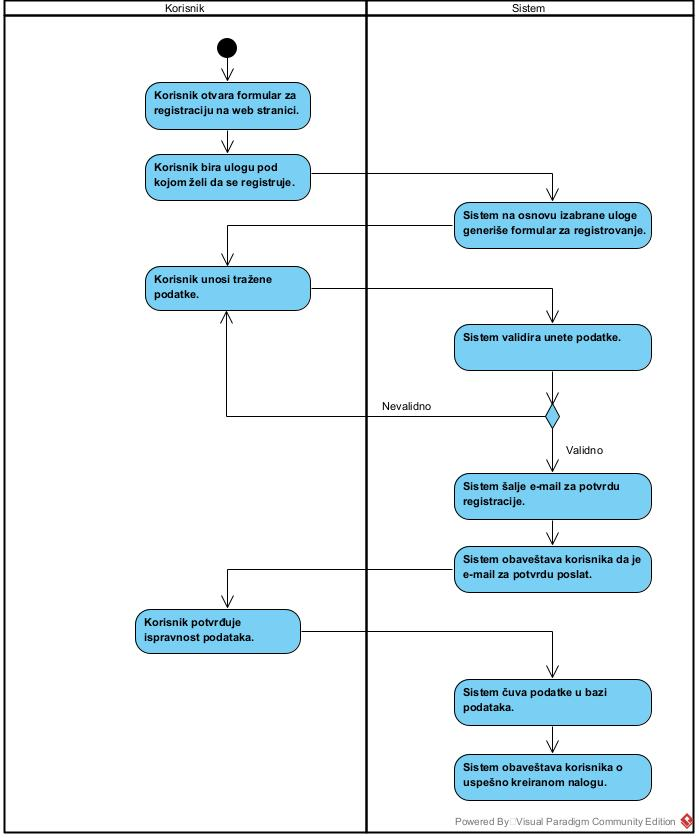
\includegraphics[scale=0.6]{Registracija_korisnika.jpg}
\caption{Registracija korisnika}
\label{slk:dtp}
\end{figure}

\newpage

\subsection{Autorizacija}
\begin{itemize}
    \item \textbf{Kratak opis:} Svi registrovani korisnici sistema, mogu se prijaviti i koristiti funkcije sistema. Neautorizovani korisnici sistema mogu ostvariti jedino funkciju čitanja vesti.
    \item \textbf{Preduslovi:} Sistem je aktivan i korisnik ima registrovan nalog.
    \item \textbf{Postuslovi:} Po uspešnoj autorizaciji, korisnik može da koristi sve funkcionalnosti sistema definisane njegovom ulogom.
    \item \textbf{Osnovni tok:}
        \begin{enumerate}
            \item Korisnik otvara web stranicu za prijavljivanje.
            \item Korisnik unosi tražene podatke.
            \item Sistem validira unete podatke.
            \item Sistem obaveštava korisnika o uspešnoj prijavi.
            \item Sistem otvara novu sesiju za prijavljenog korisnika.
            \item Sistem otvara početnu stranicu na osnovu uloge korisnika.
	    \end{enumerate}
    \item \textbf{Alternativni tokovi:}
        \begin{itemize}
            \item[A1.] \textbf{Neuspešna validacija podataka.} U slučaju pogrešno unetih kredencijala za prijavljivanje, sistem obaveštava korisnika o neispravnosti unetih podataka.
            \item[A2.] \textbf{Veliki broj neuspelih pokušaja prijavljivanja.} U slučaju da je korisnik uneo pogrešne kredencijale određen broj puta, sistem ne dozvoljava ponovni unos podataka za prijavu do isteka određenog vremenskog perioda. Sistem obaveštava korisnika o trajanju perioda nemogućnosti prijavljivanja.
        \end{itemize}
    \item \textbf{Specijalni zahtevi:}
        \begin{itemize}
			\item U slučaju da se korisnik prijavio sa novog uređaja, sistem šalje e-mail za potvrdu autentičnosti korisnika.
		\end{itemize}
	\item \textbf{Dodatne informacije:}
        \begin{itemize}
            \item  Podaci potrebni za prijavu radnika:
                \begin{itemize}
                    \item korisničko ime
                    \item broj radne knjižice
                    \item lozinka
                \end{itemize}
             \item  Podaci potrebni za prijavu čitaoca:
                \begin{itemize}
                    \item korisničko ime
                    \item lozinka
                \end{itemize}
        \end{itemize}
\end{itemize}


\begin{figure}[htbp!]
    \centering
    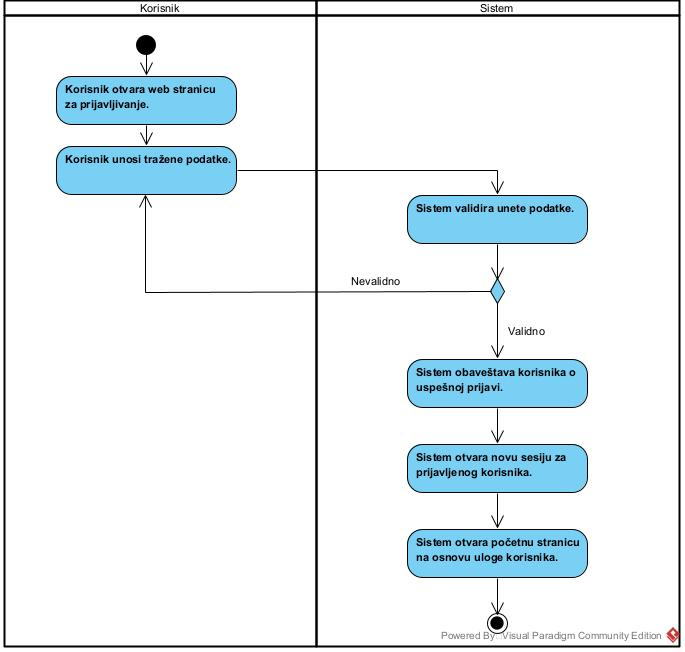
\includegraphics[scale=0.6]{Autorizacija_korisnika.jpg}
    \caption{Autorizacija korisnika}
    \label{slk:dtp}
\end{figure}

\newpage

\subsection{Slanje vesti}
\begin{itemize}
    \item \textbf{Kratak opis:} Korisnici koji su se autorizovali kao novinar ili urednik imaju mogućnost slanja vesti, što podrazumeva slanje autorskog teksta i eventualnog priloga (slika ili video) sa ciljem da se vest objavi. 
    \item \textbf{Preduslovi:} Sistem je aktivan. Korisnik je prijavljen na nalog koji ima mogućnost slanja vesti.  
    \item \textbf{Postuslovi:} Vest je skladištena u privremenu bazu i čeka odobrenje. Korisnik dobija obaveštenje da je vest pristigla.
    \item \textbf{Osnovni tok:}
        \begin{enumerate}
            \item Korisnik otvara web stranicu za slanje vesti.
            \item Korisnik prilaže vest.
            \item Sistem prihvata pristiglu vest i smešta je u bazu vesti koje su na čekanju.
            \item Sistem obaveštava korisnika o prispeću vesti i njenom statusu.
	    \end{enumerate}
    \item \textbf{Alternativni tokovi:}
        \begin{itemize}
            \item[A1.] \textbf{Korisnik nije autorizovan.} U slučaju da korisnik pokuša da pristupi stranici za slanje vesti, a prethodno se nije prijavio, sistem preusmerava korisnika na stranicu za autorizciju.
            \item[A2.] \textbf{Korisnik je poslao vest bez sadržaja.} U slučaju da je korisnik pokušao da pošalje vest koja nema sadržinu, sistem ga obaveštava o ovoj nepravilnosti.
        \end{itemize}
    \item \textbf{Dodatne informacije:}
        \begin{itemize}
            \item  Podaci koje korisnik prilaže:
                \begin{itemize}
                    \item Autorski tekst (obavezno)
                    \item Slika
                    \item Video zapis
                \end{itemize}
        \end{itemize}
\end{itemize}

\begin{figure}[htbp!]
    \centering
    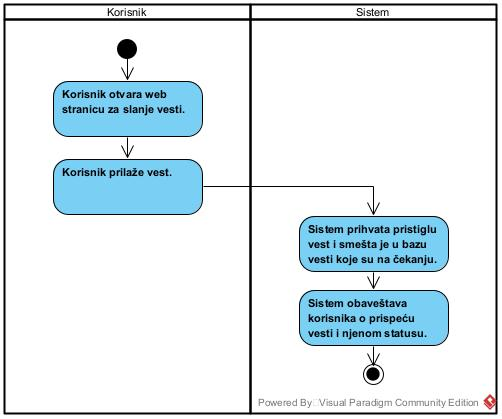
\includegraphics[scale=0.7]{Slanje_vesti.jpg}
    \caption{Slanje vesti}
    \label{slk:dtp}
\end{figure}

\newpage

\subsection{Pretraživanje vesti i tema}
\begin{itemize}
    \item \textbf{Kratak opis:} Sistem omogućava korisnicima autorizovanim sa ulogama: novinar, urednik i administrator da pretražuju objavljene vesti, i spiskove tema na kojima rade ostali novinari. Cilj pretrage je da se spreči ponavljanje tema na koje novinari pišu kao i da se iskoriste već postojeće vesti.  
    \item \textbf{Preduslovi:} Sistem je aktivan. Korisnik je autorizovan sa odgovarajućom ulogom. 
    \item \textbf{Postuslovi:} Korisnik dobija listu vesti ili tema koje ispunjavaju uslove pretrage.
    \item \textbf{Osnovni tok:}
        \begin{enumerate}
            \item Korisnik otvara web stranicu za pretraživanje.
            \item Korisnik unosi uslove po kojima želi da filtrira pretragu.
            \item Sistem obrađuje unete uslove i iz baze podataka vraća listu koja odgovara uslovima pretrage.
            \item Sistem šalje dobijenu listu korisniku.
            \item Korisnik može da nastavi ili da završi pretragu.
	    \end{enumerate}
    \item \textbf{Alternativni tokovi:}
        \begin{itemize}
            \item[A1.] \textbf{Korisnik nije autorizovan.} U slučaju da korisnik pokuša da pristupi stranici za pretraživanje vesti, pri čemu nije prijavljen, sistem preusmerava korisnika na stranicu za autorizciju.
            \item[A2.] \textbf{Za unete uslove pretrage ne postoje entiteti koji ih ispunjavaju.} U slučaju da ne postoje entiteti koji ispunjavaju uslove pretrage, sistem obaveštava korisnika o nastaloj situaciji.
        \end{itemize}
    \item \textbf{Specijalni zahtevi:}
        \begin{itemize}
			\item Neophodno je uneti bar jedan uslov pretrage.
		\end{itemize}
	\item \textbf{Dodatne informacije:}
        \begin{itemize}
            \item Pretragu je moguće vršiti po:
                \begin{itemize}
                    \item Vrsti pretrage (da li se vrši pretraga vesti ili tema)
                    \item Naslovu vesti
                    \item Oblasti u kojoj se nalazi vest
                    \item Datumu objavljivanja vesti
                    \item Autoru vesti
                    \item Ključnim rečima u tekstu vesti
                \end{itemize}
        \end{itemize}
\end{itemize}

\begin{figure}[htbp!]
    \centering
    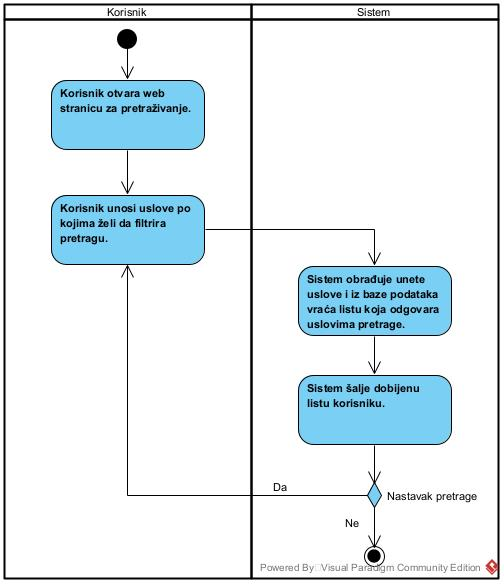
\includegraphics[scale=0.7]{Pretrazivanje_vesti_i_tema.jpg}
    \caption{Pretrazivanje vesti i tema}
    \label{slk:dtp}
\end{figure}

\newpage

\subsection{Manipulacija vestima u bazi}
\begin{itemize}
    \item \textbf{Kratak opis:} Sistem omogućava korisnicima autorizovanim sa ulogom urednika da manipulišu(ispravlaju, dopunjuju, brišu) svim vestima u bazi.
    \item \textbf{Preduslovi:} Sistem je aktivan. Korisnik je autorizovan sa odgovarajućom ulogom. 
    \item \textbf{Postuslovi:} Izmenjene vesti su uspešno sačuvane u bazi sa svojim izmenama.
    \item \textbf{Osnovni tok:}
        \begin{enumerate}
            \item Korisnik otvara web stranicu koja mu daje uvid u sve vesti
	        \item Korisnik pretražuje vesti
	        \item Sistem vraća korisniku vesti koje odgovaraju uslovima pretrage
	        \item Korisnik bira vest kojom želi da manipuliše
	        \item Korisnik potvrđuje da napravljene izmene budu trajno sačuvane
	        \item Sistem napravljene promene čuva u bazi podataka
	    \end{enumerate}
    \item \textbf{Alternativni tokovi:}
        \begin{itemize}
            \item[A1.] \textbf{Korisnik nije napravio nijednu izmenu nad vestima koje je izabrao.} U slučaju da korisnik ipak nije izmenio vest, prilikom slanja zahtev da se vest sačuva sistem ga obaveštava o tome. Korisnik se zatim vraća na stranicu gde se nalaze sve vesti a sistem ne ažurirara podatke u bazi(vreme poslednje modifikacije, razlog poslednje izmene...).
        \end{itemize}
    \item \textbf{Specijalni zahtevi:}
        \begin{itemize}
			\item Prilikom menjanja određene vesti, potrebno je uneti i razlog zbog kog se ta izmena pravi.
		\end{itemize}
\end{itemize}

\begin{figure}[htbp!]
    \centering
    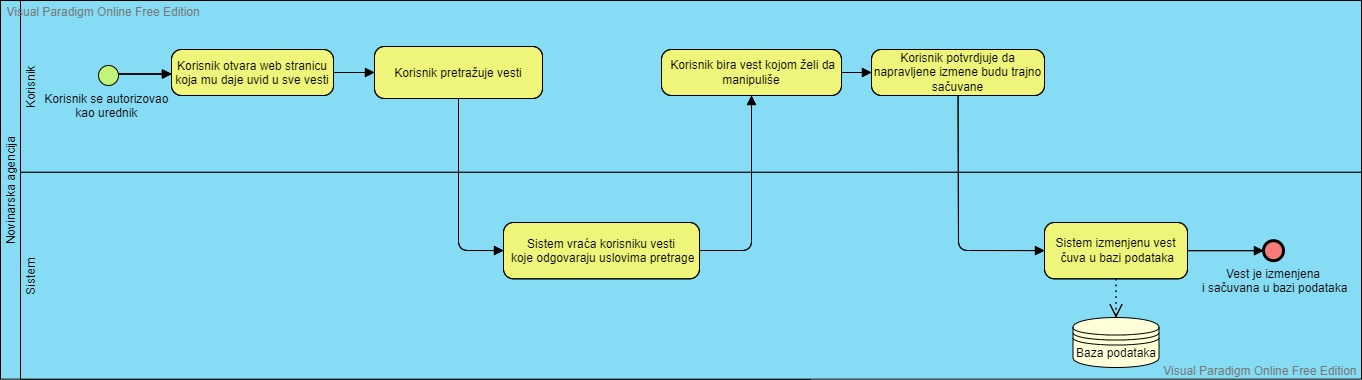
\includegraphics[scale=0.3]{Manipulacija_vestima_u_bazi.jpg}
    \caption{Manipulacija vestima u bazi}
    \label{slk:dtp}
\end{figure}

\newpage

\subsection{Selekcija vesti}
\begin{itemize}
    \item \textbf{Kratak opis:} Sistem omogućava korisnicima autorizovanim sa ulogom urednika da vrši odabir napisanih vesti koje su na čekanju. Ukoliko urednik da odobrenje za određenu vest, ona će biti i objavljena.
    \item \textbf{Preduslovi:} Sistem je aktivan. Korisnik je autorizovan sa odgovarajućom ulogom. 
    \item \textbf{Postuslovi:} Rešen je status napisanih vesti koje su bile na čekanju.
    \item \textbf{Osnovni tok:}
        \begin{enumerate}
            \item Korisnik otvara web stranicu na kojoj može videti sve vesti
            \item Korisnik pretražuje vesti koje čekaju na odobrenje
            \item Sistem vraća korisniku tražene vesti iz baze podataka
            \item Korisnik radi selekciju vesti
            \item Sistem beleži promene statusa vesti i izmene čuva u bazi podataka
        \end{enumerate}
    \item \textbf{Alternativni tokovi:}
        \begin{itemize}
            \item[A1.] \textbf{Ne postoje vesti na čekanju} Ukoliko nema vesti koje čekaju odobrenje, sistem obaveštava korisnika o tome. 
        \end{itemize}
    \item \textbf{Specijalni zahtevi:}
        \begin{itemize}
			\item Ukoliko vest nije dobila odobrenje, potrebno je da se navede razlog zbog kog se to desilo.
		\end{itemize}
	\item \textbf{Dodatne informacije:}
        \begin{itemize}
            \item Neki od glavnih kriterijuma selekcije vesti mogu biti:
                \begin{itemize}
                    \item Istinitost
                    \item Potpunost
                    \item Javni značaj 
                    \item Objektivnost
                \end{itemize}
        \end{itemize}
\end{itemize}


\begin{figure}[htbp!]
    \centering
    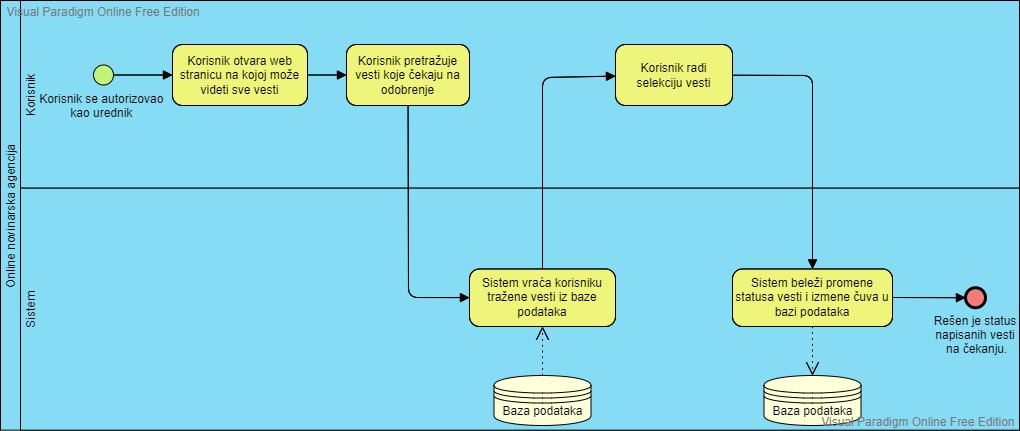
\includegraphics[scale=0.35]{Selekcija_vesti.jpg}
    \caption{Selekcija vesti}
    \label{slk:dtp}
\end{figure} 

\newpage

\section{Baza podataka}
Na osnovu definisanih slučajeva upotrebe, primećene su sledeće grupe podataka koje bi trebalo smestiti u bazu:
\begin{itemize}
    \item Nalog
    \item Zaposleni
        \begin{itemize}
            \item Novinar
            \item Urednik
            \item Administrator 
        \end{itemize}
    \item Čitalac
    \item Vest
    \item Komentar
    \item Ocena
\end{itemize}

\subsection{Podaci o nalogu}
Obzirom da svaki korisnik mora kreirati nalog kako bi učestvovao u sistemu jasno je da se podaci neophodni za kreiranje naloga moraju zajedno grupisati. \\

Podaci o nalogu koji se čuvaju su:
\begin{itemize}
    \item id
    \item ime
    \item prezime
    \item email
    \item korisničko ime
    \item lozinka
\end{itemize}

Klasa nalog može se konkretizovati klasama zaposleni(nalozi sa specijalnim mogućnostima) i čitalac. Ova klasa vezuje se i sa klasom administrator, jer administratori mogu upravljati nalozima.

\subsection{Podaci o zaposlenom}
Zaposleni predstavlja konkretizaciju naloga. Zaposleni imaju naloge sa specijalizovanim ulogama.

Podaci o zaposlenima koji se čuvaju:
\begin{itemize}
    \item broj radne knjižice
    \item broj telefona
\end{itemize}

\subsection{Novinar}

Novinar predstavlja konkretizaciju zaposlenog. Obzirom na svoju ulogu u sistemu(pisanje vesti), novinar od dodatnih podataka sadrži samo \textbf{id vesti} kako bi se moglo definisati koje vesti je napisao dati novinar

\subsection{Urednik}

Urednik predstavlja konkretizaciju zaposlenog. Kao i u slučaju novinara, jedino proširenje u pogledu podataka urednik ostvaruje jednim dodatnim atributom: \textbf{id vesti}. Kroz ovaj atribut urednik se povezuje sa vestima i ostvaruje mogućnosti kreiranja vesti, menjanja njenog statusa, korigovanja komentara vesti i sl.

\subsection{Administrator}

Administrator predstavlja konkretizaciju zaposlenog. Obzirom da je glavna uloga administratora upravljanje nalozima, ova grupa podataka ne zahteva nikakva proširenja skupa atributa. Administrator se vezuje jedino sa klasom nalog, i tako direktno utiče na upravljanje njima. 

\subsection{Vesti}

Centralna klasa celog sistema je klasa vest. Od podataka, ova klasa čuva:

\begin{itemize}
    \item id vesti
    \item id novinara
    \item id komentara
    \item id ocena
    \item tekst
    \item kategorija
    \item vreme
    \item mesto
    \item status
\end{itemize}

Obzirom da ostvaruje vezu sa klasama: novinar, komentar i ocena, ova klasa sadrži identifikatore klasa sa kojima se vezuje. Kako bi se znalo koji novinar je napisao vest, koje komentare vest sadrži i sa kojim ocenama je vest ocenjena neophodno je da se uspostavi veza ovih klasa sa klasom vest. \\
Kao osnovne atribute vest sadrži tekst, prilog(dodatak), vreme kada je vest napisana i mesto na kojem je nastala. Takođe, vest treba da sadrži kategoriju kojoj pripada i to sa nekom od predefinisanih mogućnosti:

\begin{itemize}
    \item aktuelnosti
    \item zabava
    \item biznis
    \item hronika
    \item politika
    \item drustvo
    \item svet
    \item nauka
    \item umetnost
    \item IT
    \item sport
    \item ostalo  
\end{itemize}

\  \\

\indent Zavisno od tekućeg stanja u kojem se vest nalazi, status moze imati neku od sledećih vrednosti:
\begin{itemize}
    \item u pripremi
    \item na čekanju
    \item odobrena
    \item arhivirana
\end{itemize}



\subsection{Komentar}

Obzirom da je ovaj sistem izrazito dinamičan, postavljanje komentara je jedna od najčešćih operacija koja se događa u sistemu. S tim u vezi, kao jako značajna klasa izdvaja se klasa komentar. Ova klasa čuva naredne podatke:

\begin{itemize}
    \item id komentara
    \item id naloga
    \item id vesti
    \item id ocena
    \item tekst
    \item vreme
\end{itemize}

Svaki komentar, mora znati za: nalog koji ga je kreirao i vest na koju se komentar odnosi. Takođe komentar može biti ocenjen od strane drugih korinika sistema, pa je neophodno ostvariti vezu i sa klasom ocena. Poredm toga, komentar sadrži i osnovne podatke poput teksta komentara i vremena kada je komentar objavljen.   

\subsection{Ocena}

Kao još jedan vid povratne infomacije od čitalaca, imamo i ocene koje čitaoci mogu ostavljati za vesti ili komentare drugih čitalaca. Od podataka, klasa ocena čuva:

\begin{itemize}
    \item id ocene
    \item id čitaoca
    \item id objekta(vesti ili komentara)
    \item vrednost
    \item tip(na šta se odnosi ocena: vest ili komentar)
\end{itemize}

\subsection{Čitalac}

Čitaoc predstavlja konkretizaciju naloga. Njegova uloga u sistemu jeste čitanje vesti uz omogućenu interakciju kroz ocene i komentare. 

Podaci o čitaocu koji se čuvaju su:
\begin{itemize}
    \item id čitaoca
    \item id komentara
    \item id ocena
\end{itemize}


\begin{figure}[htbp!]
    \centering
    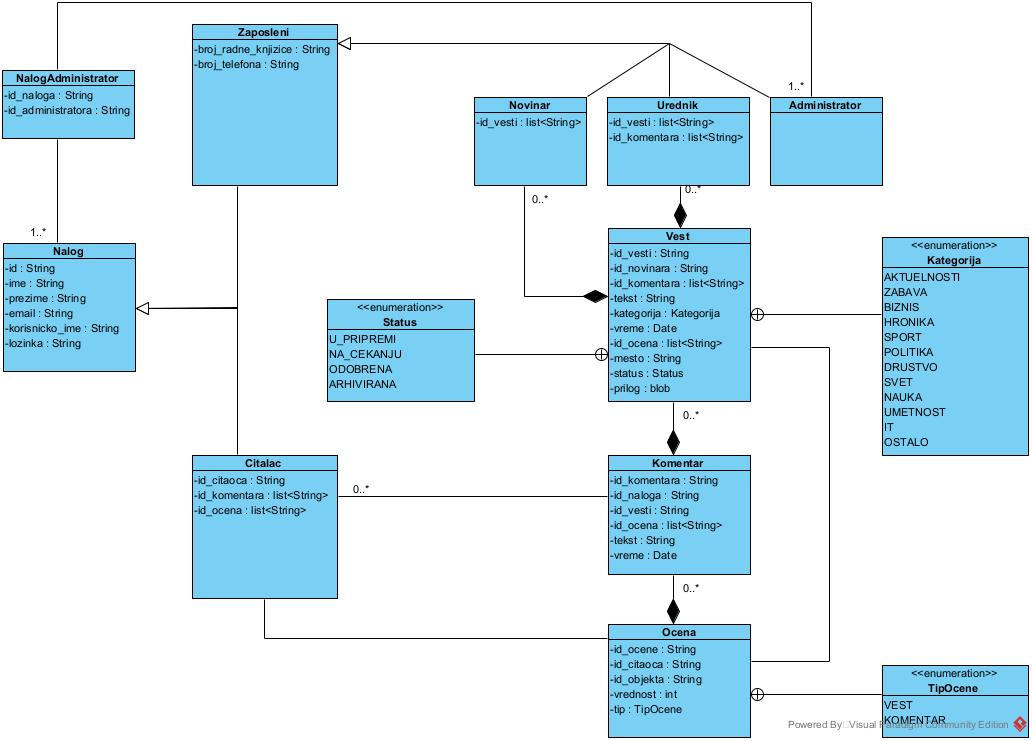
\includegraphics[scale=0.4]{Dijagram_klasa.jpg}
    \caption{Dijagram klasa podataka}
    \label{slk:dtp}
\end{figure}

\newpage

\section{Softverska arhitektura}

Posmatrani informacioni sistem ima tri osnovna podsistema:

\begin{enumerate}
    \item \textbf{Zaposleni} - omogućava korišćenje sistema od strane novinara i urednika pri čemu se koriste usluge sledećih komponenti:
        \begin{itemize}
            \item Autentikacija - omogućava kreiranje novih naloga i registraciju zaposlenih sa već kreiranim nalozima
            \item Obrada vesti - omogućava slanje, odobravanje vesti od strane urednika, pretraživanje vesti i tema, manipulaciju vestima koje su u bazi
            \item Obrada komentara - omogućvava uklanjanje i izmenjivanje komentara
        \end{itemize}
    \item \textbf{Čitalac} - omogućava korišćenje sistema od strane čitalaca pri čemu se koriste usluge sledećih komponenti:
        \begin{itemize}
            \item Autentikacija - omogućava kreiranje novih naloga i registraciju zaposlenih sa već kreiranim nalozima
            \item Čitanje vesti - omogućvava pretraživanje i čitanje vesti
            \item Pisanje komentara i ocenjivanje - omogućvava postavljanje komentara i ocenjivanje vesti
        \end{itemize}
    \item \textbf{Administrator} - omogućava korišćenje sistema od strane administratora pri čemu se koriste usluge sledećih komponenti:
        \begin{itemize}
            \item Administracija - omogućava pre svega manipulaciju nalozima u bazi
        \end{itemize}
\end{enumerate}

Takođe, nabrojane komponente koriste bazu podataka posredstvom interfejsa za komunikaciju sa bazom podataka(JDBC).  

\begin{figure}[htbp!]
    \centering
    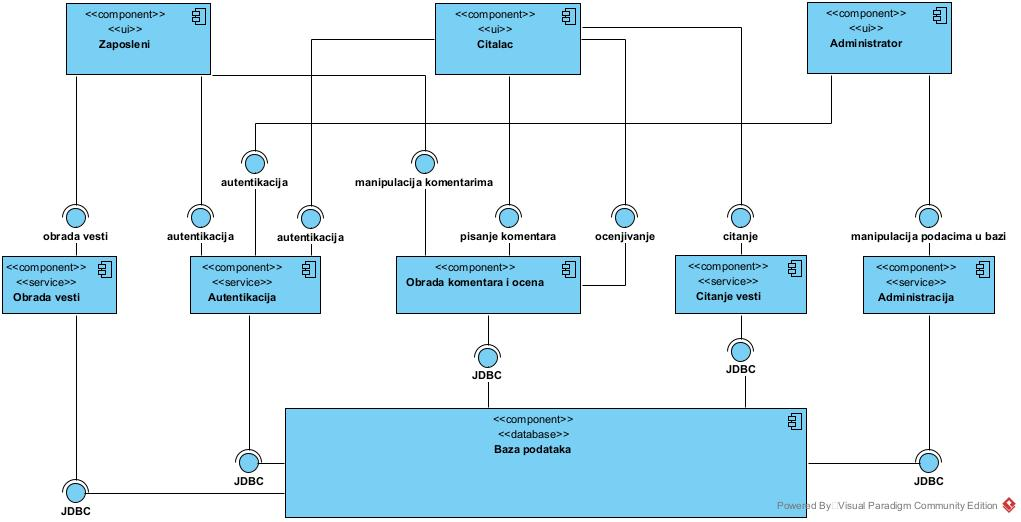
\includegraphics[scale=0.38]{Dijagram_komponenti.jpg}
    \caption{Dijagram komponenti}
    \label{slk:dtp}
\end{figure}

\newpage

\newpage

Informacioni sistem je podeljen na aplikacioni server i server baze podataka koji međusobno komuniciraju putem TCP/IP protokola. Aplikacioni server koristi JSP server Tomcat 10 i na njemu se izvršava aplikacija \textit{novinarska\_agencija.war}.
Što se same implementacije tiče, \textit{zaposleni.jar} implementira komponentu zaposleni, \textit{citalac.jar} implementira komponentu citalac, a \textit{administrator.jar} implementira komponentu administrator. Za konfigurisanje aplikacije korišćen je fajl
\textit{web\_config.xml}. Na serveru baze podataka se nalazi sama baza i radno okruženje \textit{MySQL}. 

\begin{figure}[htbp!]
    \centering
    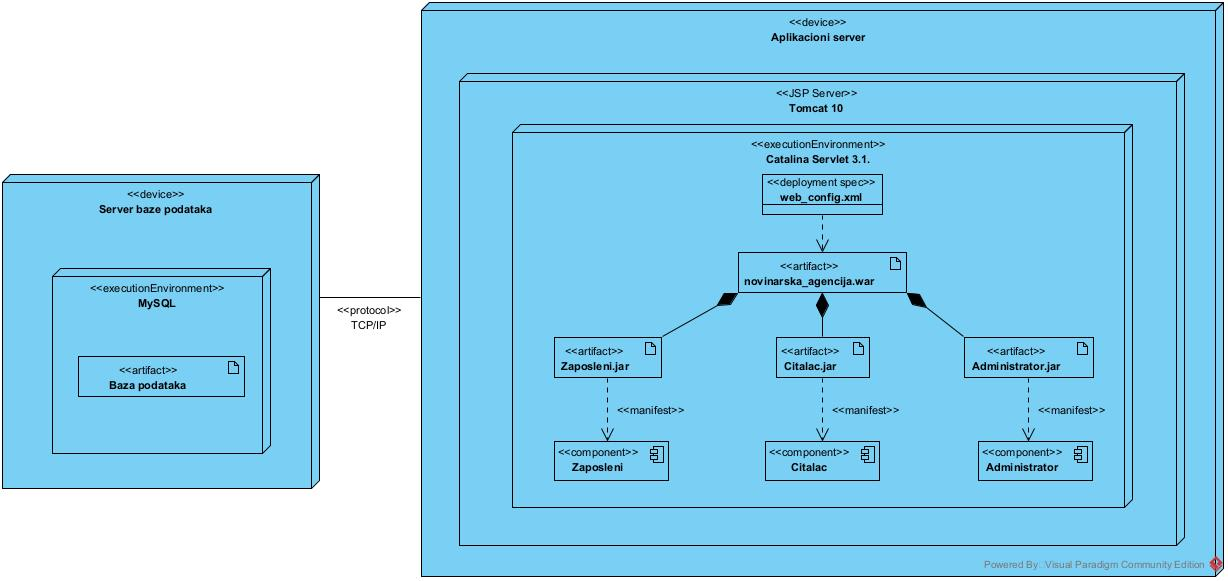
\includegraphics[scale=0.33]{Dijagram_isporucivanja.jpg}
    \caption{Dijagram isporucivanja}
    \label{slk:dtp}
\end{figure}


\newpage
\section{Korisnički interfejs}

\begin{figure}[htbp!]
    \centering
    
\includegraphics[scale=0.20]{PrijavaCitalaca.png}
    \caption{Prijavljivanje čitalaca}
    \label{slk:dtp}
\end{figure}

\begin{figure}[htbp!]
    \centering
    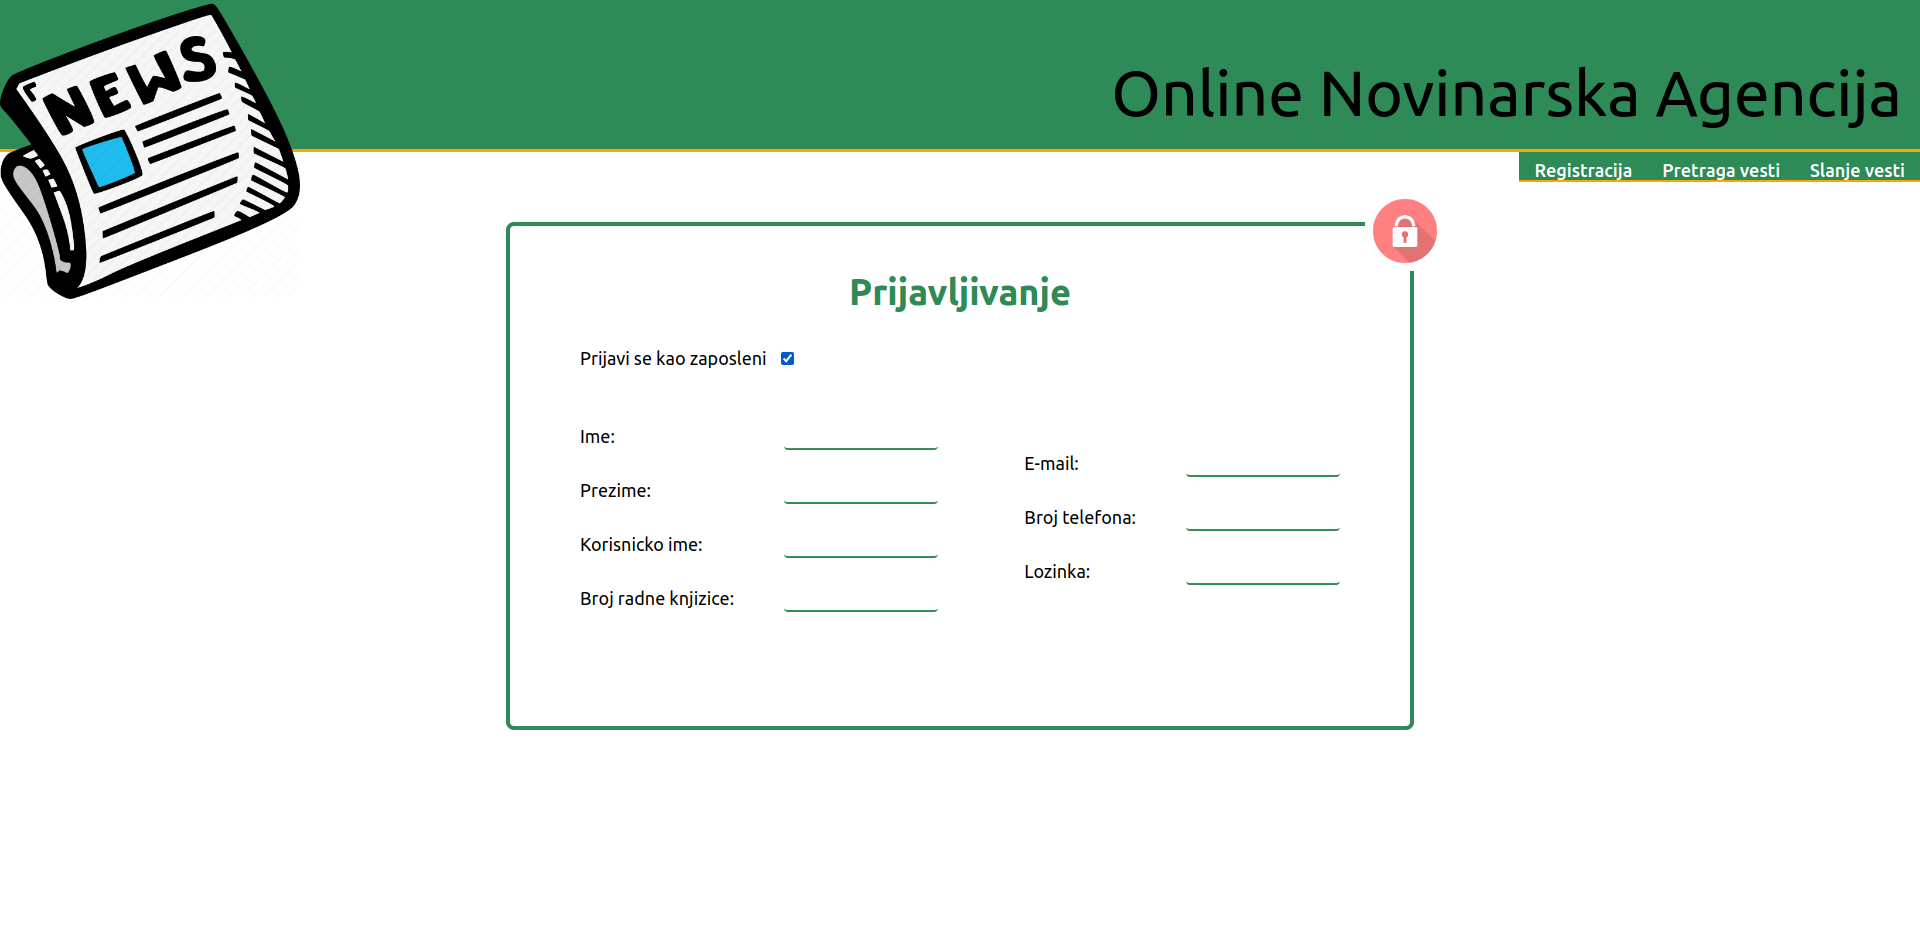
\includegraphics[scale=0.20]{PrijavljivanjeRadnika.png}
    \caption{Prijavljivanje radnika}
    \label{slk:dtp}
\end{figure}

\begin{figure}[htbp!]
    \centering
    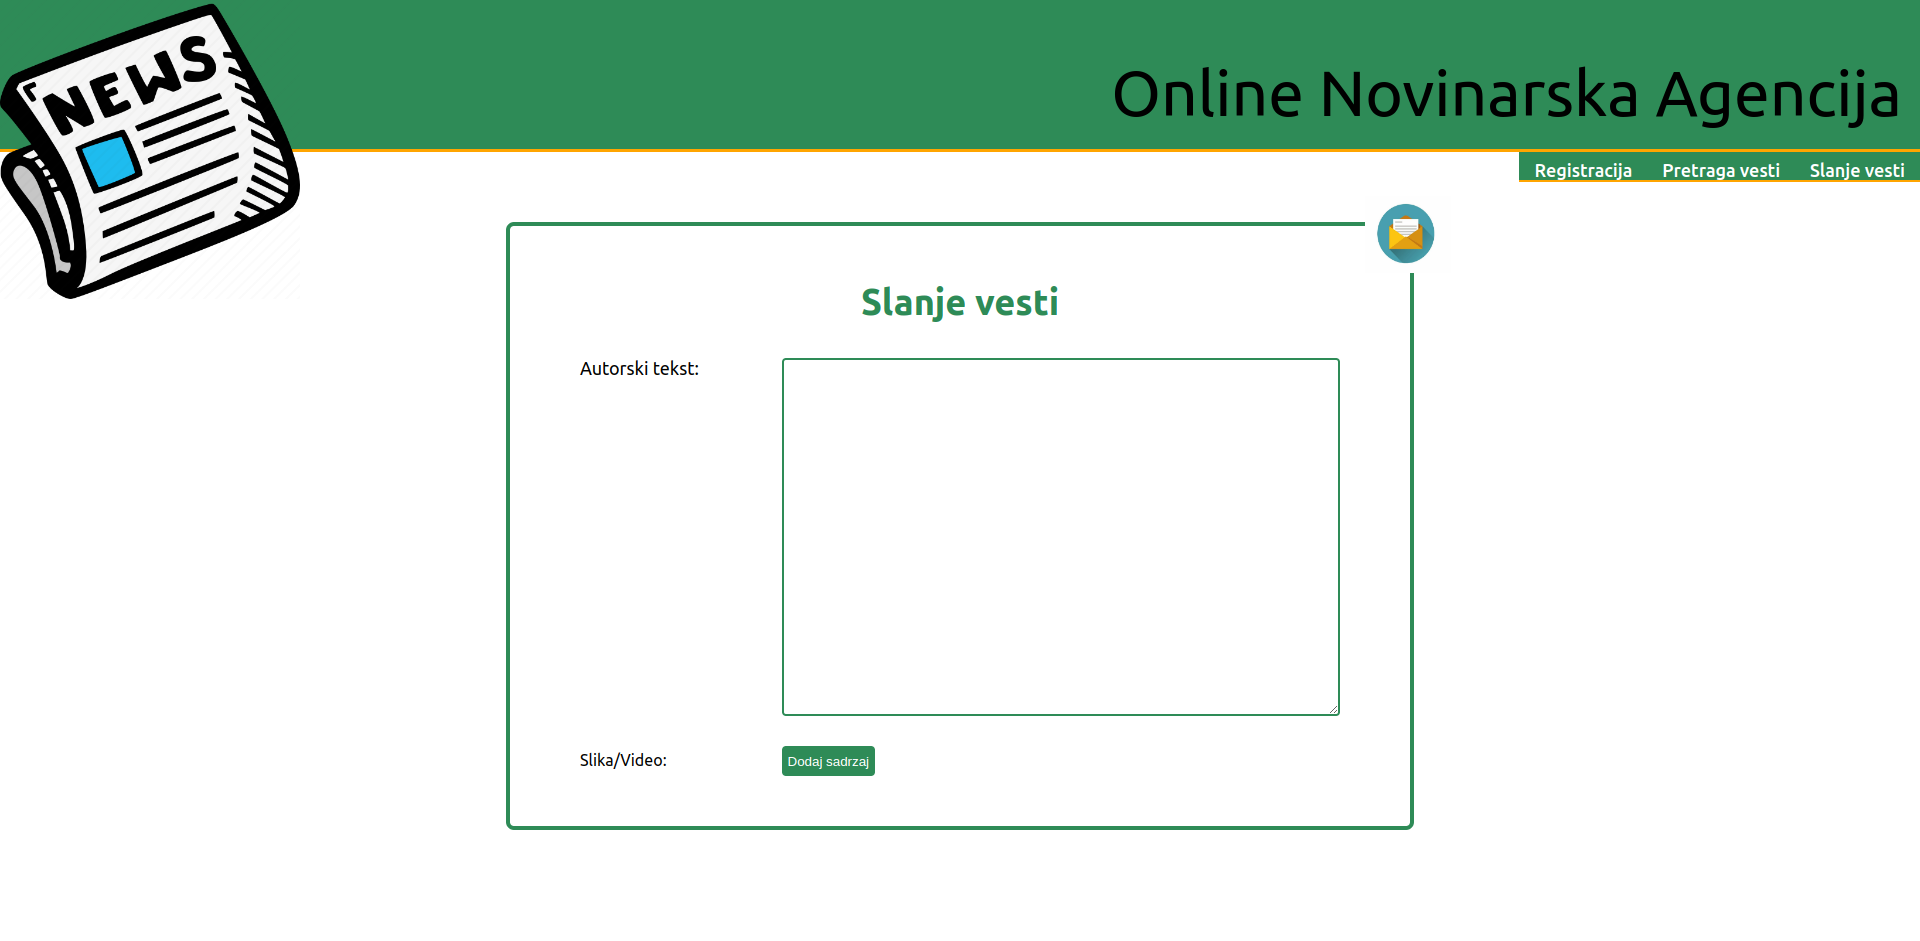
\includegraphics[scale=0.20]{SlanjeVesti.png}
    \caption{Slanje novih vesti}
    \label{slk:dtp}
\end{figure}

\begin{figure}[htbp!]
    \centering
    \includegraphics[scale=0.20]{PregledVesti.png}
    \caption{Pregled svih vesti}
    \label{slk:dtp}
\end{figure}

\begin{figure}[htbp!]
    \centering
    \includegraphics[scale=0.20]{PrimerVesti.png}
    \caption{Primer otvorene vesti}
    \label{slk:dtp}
\end{figure}
\end{document}
